\documentclass[11pt,letterpaper]{article}
\usepackage[letterpaper,margin=0.65in,includefoot,headheight=14pt,footskip=0.30in]{geometry}
\usepackage[T1]{fontenc}
\usepackage{lmodern,microtype}
\usepackage{booktabs,tabularx,array}
\usepackage{graphicx,xcolor}
\usepackage{tikz}
\usetikzlibrary{arrows.meta,positioning}
\usepackage{caption,enumitem,needspace,float}
\usepackage{fancyhdr}
\usepackage[hidelinks]{hyperref}
\definecolor{ink}{HTML}{173D39}
\definecolor{teal}{HTML}{26786C}
\definecolor{pale}{HTML}{EDF5F1}
\definecolor{muted}{HTML}{525D60}
\hypersetup{pdftitle={Helping Hand: R3 Preliminary Report},pdfauthor={Brian Paz, Gael Garcia, Kali Schuchhardt, Srinitha Srikanth}}
\setlength{\parindent}{0pt}
\setlength{\parskip}{3pt plus 1pt minus 1pt}
\setlength{\emergencystretch}{2em}
\setlength{\tabcolsep}{5pt}
\renewcommand{\arraystretch}{1.12}
\captionsetup{font=small,labelfont=bf,justification=raggedright,singlelinecheck=false}
\setlist{nosep,leftmargin=*}
\newcolumntype{Y}{>{\raggedright\arraybackslash}X}
\newcolumntype{P}[1]{>{\raggedright\arraybackslash}p{#1}}
\pagestyle{fancy}
\fancyhf{}
\fancyfoot[L]{\footnotesize\color{muted}HELPING HAND \textbar{} CEN4908C \textbar{} R3}
\fancyfoot[R]{\footnotesize\color{muted}\thepage}
\renewcommand{\headrulewidth}{0pt}
\renewcommand{\footrulewidth}{0.3pt}
\raggedbottom

\begin{document}
{\LARGE\bfseries\color{ink}Helping Hand\par}
{\large Preliminary Report: Wearable-Assisted ASL Learning\par}
\smallskip
{\small Brian Paz, Gael Garcia, Kali Schuchhardt, Srinitha Srikanth\\
Computer Engineering, CEN4908C \hfill October 28, 2026\\
Evidence cutoff: October 28, 2026\par}
\vspace{4pt}
\hrule
\vspace{5pt}

% ABSTRACT START
\section*{Abstract}
Helping Hand is a wearable-assisted American Sign Language (ASL) learning
prototype intended to support beginner practice through sensor-based feedback
and persistent learner progress. Five resistive flex sensors and a wrist-mounted
six-axis inertial measurement unit (IMU) connect to an ESP32-S3, which streams
measurements and static predictions over Bluetooth Low Energy (BLE) to a Flutter Android application.
The application provides account access, target-specific practice, recording
and export tools, and local-first progress storage with Firebase synchronization.
This report describes the design, scientific background, preliminary results,
engineering constraints, community considerations, and remaining development.
The original 36-class static classifier is preserved as a baseline; current
firmware packages a separate 34-class model trained from recorded poses.
For isolated words, a temporal convolutional network (TCN) was compared with
two convolutional/recurrent alternatives using fifteen real recordings of Hello,
Please, and Yes. All candidates correctly classified three validation trials;
the TCN was selected by the predefined model-size tie-break at 48,324 bytes
and subsequently classified three reserved test trials correctly. These small,
neutral-orientation results do not establish performance across users or live
conditions. Software checks and Android recorded replay support integration,
while current physical validation remains incomplete. Two damaged
flex sensors have delayed reliable new data collection. Replacement flex sensors
remain awaited; the nine-axis IMU and piezo elements have been received for
planned orientation sensing and tactile feedback. Near-term work addresses
sensor repair, calibration, printed circuit board (PCB) development, recognition robustness, haptic
cue mapping, and reproducible end-to-end testing. Educational effectiveness
and reliable corrective feedback remain objectives requiring user evaluation.
% ABSTRACT END

% BODY START
\section{Introduction}
Learning ASL requires practice of handshape, movement, orientation, location
and nonmanual features. ASL is a natural language with grammar distinct from
English; it is not a universal sign system~\cite{nidcd}. Helping Hand explores whether a portable sensor
glove and companion application can make independent beginner practice more
informative between interactions with instructors and fluent signers.

The original design identified hearing beginners as intended learners and
proposed tactile correction, modular hardware and structured practice~\cite{design}.
The prototype combines recognition and saved practice; corrective haptics remain
under development.
A recent study involving ASL educators identifies structured signing feedback
as a useful technology direction while emphasizing pedagogical and cultural
considerations~\cite{educators}. Helping Hand therefore targets a bounded
learning aid; recognition of selected signs alone cannot demonstrate ASL
competence or improved learning.

\section{Background and Technical Basis}
A static classifier maps a single sensor vector to a label. Moving signs
require temporal structure: the order and duration of observations can
distinguish gestures that share individual poses. Lee, Chong and Chung
demonstrated word-level ASL recognition using six IMUs and a long short-term
memory (LSTM) network~\cite{lee}. That study supports feasibility, but its fingertip sensing,
dataset and evaluation differ from Helping Hand's five flex sensors and single
wrist IMU. Published accuracy is not transferable to this prototype.

TCNs use temporal convolutions to combine neighboring observations; dilation
extends the temporal context without a recurrent state. Bai, Kolter and Koltun
provide a general comparison of convolutional and recurrent sequence models
in an author preprint~\cite{tcn}. Helping Hand compares TCN, CNN-GRU and
CNN-LSTM on identical recordings and preprocessing. These alternatives combine
convolutional neural networks (CNNs) with gated recurrent unit (GRU) or LSTM
layers. Trial boundaries must remain intact during splitting:
neighboring frames from one sign are correlated and should not appear as
independent training and test examples.

Orientation is both a sensing problem and meaningful sign information.
Quaternion-based activity-recognition research motivates evaluating frame
transformations under sensor rotation~\cite{quaternion}; it does not prove
that removing orientation helps ASL. Accelerometer/gyroscope fusion can estimate
tilt and short-term rotation, while a calibrated magnetometer can provide a
heading reference. Kok and Sch\"on demonstrate the importance of magnetic
calibration and axis alignment~\cite{magnetic}. A magnetic reference may reduce
yaw drift, but nearby magnetic disturbances can degrade heading. The nine-axis
upgrade will test this tradeoff; no orientation normalization is implemented in the
current word demo. Haptic perception also requires testing during movement:
Tajdari, Forsyth and Lim found lower vibrotactile identification accuracy during
repetitive hand motion~\cite{hapticstudy}. Their results motivate a glove-specific
cue study, not a claim that our acquired buzzers provide effective guidance.

\section{System Design}
\subsection{Acquisition, communication and inference}
The current glove retains the demo's perfboard-based electronics assembly
(Figure~\ref{fig:prototype}). It connects five flex channels to ESP32-S3
analog inputs A0--A4 and reads its
current accelerometer/gyroscope over I\textsuperscript{2}C. Firmware targets a
40~Hz stream and records sequence numbers and device timestamps for delivery
checks. BLE notifications carry raw flex values, acceleration, angular rate,
sensor status and static predictions to one shared Flutter connection service.
The Nordic UART-style custom GATT service provides device-to-app notifications
and an app-to-device write characteristic~\cite{ble,nus}. Its text packet
contract is project-specific; the write path currently logs commands
and does not drive haptics. Sustained packet integrity still requires
target-phone measurements.

\begin{figure}[!ht]
\centering
\rotatebox[origin=c]{-90}{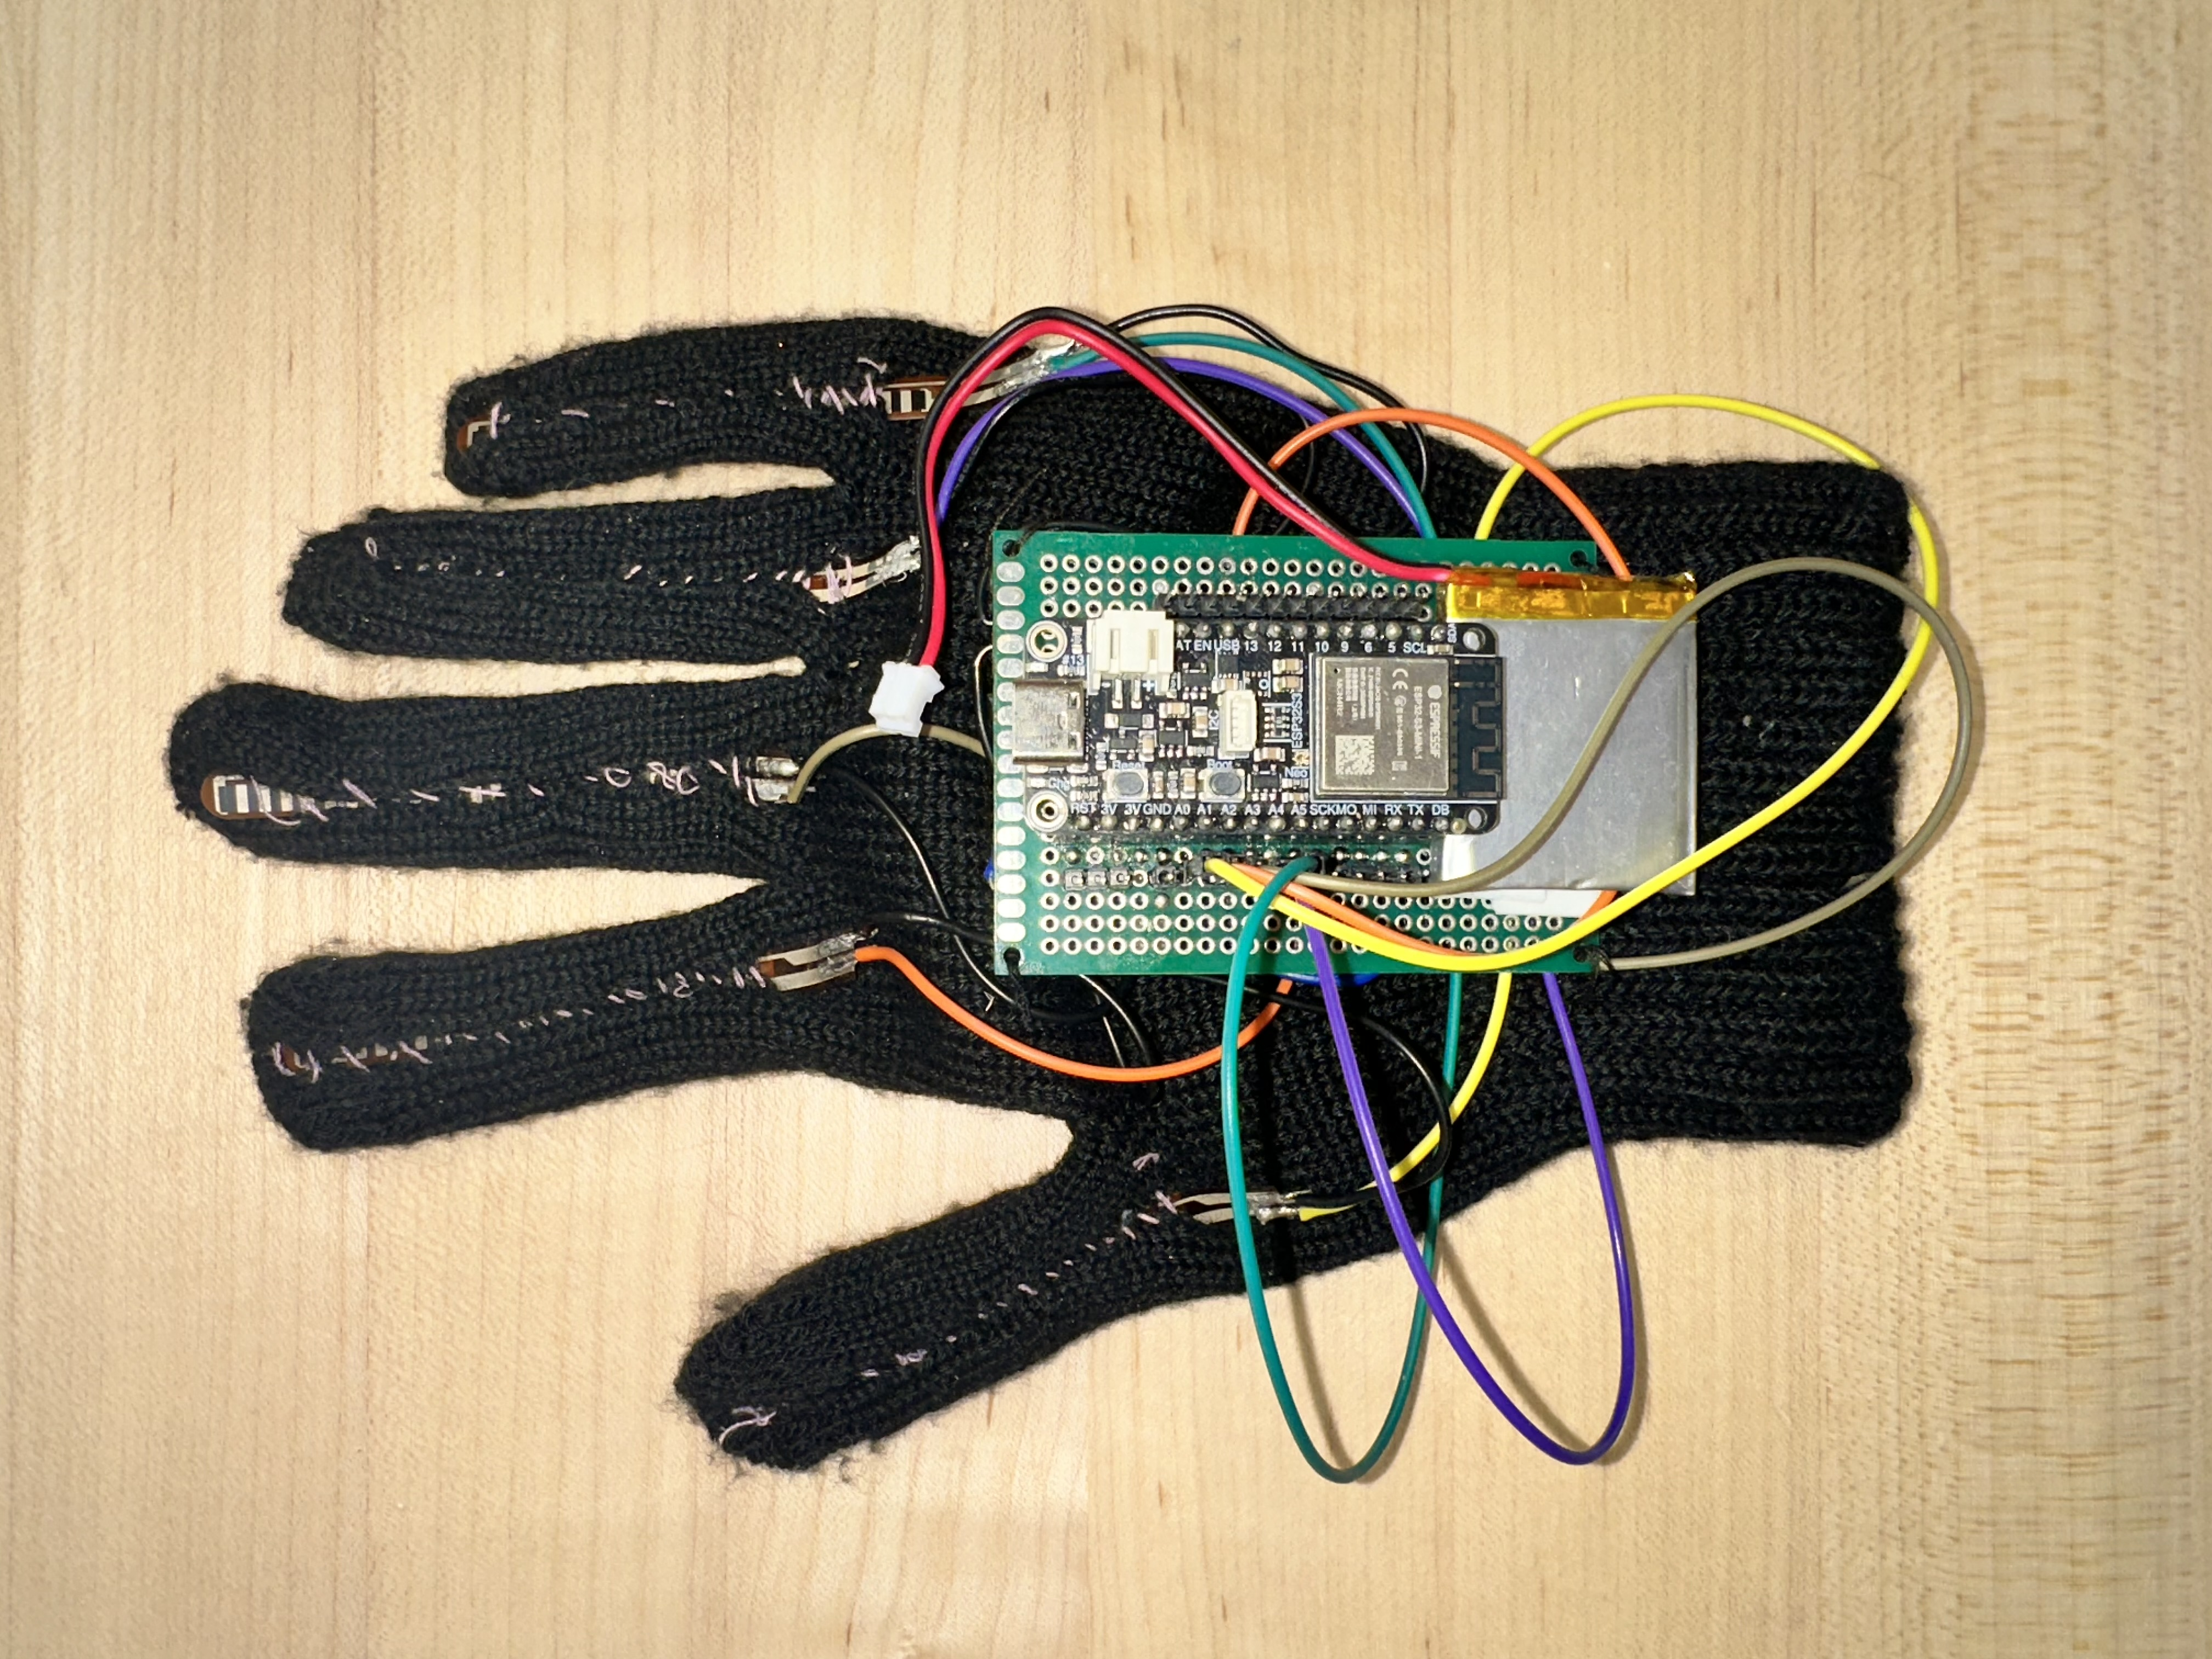
\includegraphics[width=2.85in]{../beta_presentation/assets/hardware/glove-current.jpg}}
\caption{Team prototype photograph used in the October 6 presentation: finger
sensor mounting, wiring and glove-mounted perfboard electronics~\cite{repo}.
The photograph documents assembly, not sensor health or integrated haptic feedback.}
\label{fig:prototype}
\end{figure}

The static path runs a multilayer perceptron on ESP32. Current firmware defaults
to a 34-class recorded model covering digits and letters except motion-based
J/Z; the original synthetic 36-class baseline remains separately available.
The recorded model uses five calibrated flex inputs, two hidden layers of
128 and 64 units, and a softmax output~\cite{staticrecord}.

The word path runs locally on the phone. Each complete attempt is linearly
resampled at 40~Hz using the device clock, center-trimmed or edge-padded to
96 samples (approximately 2.4 seconds),
and standardized using training-only statistics. Its eleven features are five
raw flex readings followed by three acceleration and three angular-rate
channels. A 16-filter projection feeds three residual TCN blocks with two
kernel-five causal convolutions per block and dilations 1, 2 and 4. Temporal
averaging, a 16-unit dense layer and softmax yield three word scores. Dropout
and L2 regularization are already present~\cite{wordrecord}.

\begin{figure}[H]
\centering
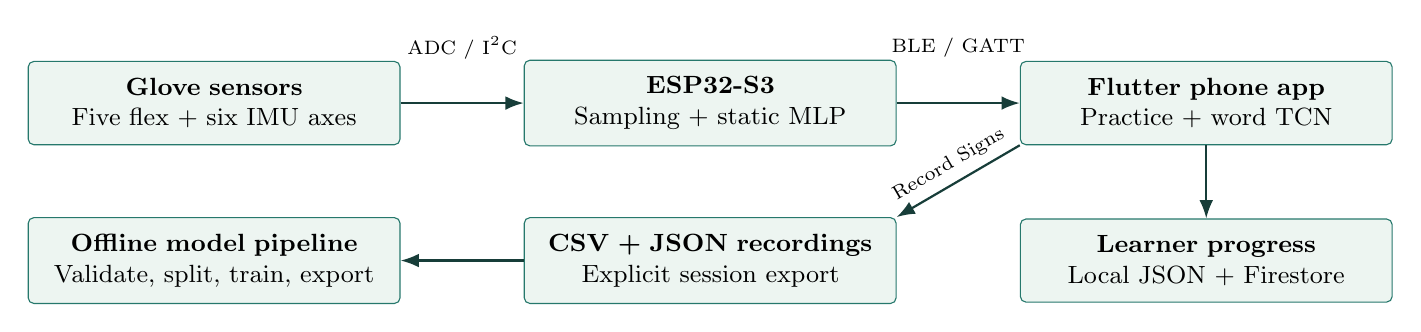
\begin{tikzpicture}[font=\small,>=Latex,
  box/.style={draw=teal,rounded corners=2pt,fill=pale,align=center,inner sep=6pt,minimum height=1.05cm},
  flow/.style={->,thick,draw=ink}]
\node[box,text width=4.3cm] (sensors) at (0,0) {\textbf{Glove sensors}\\Five flex + six IMU axes};
\node[box,text width=4.3cm] (esp) at (6.3,0) {\textbf{ESP32-S3}\\Sampling + static MLP};
\node[box,text width=4.3cm] (app) at (12.6,0) {\textbf{Flutter phone app}\\Practice + word TCN};
\draw[flow] (sensors) -- (esp);
\draw[flow] (esp) -- (app);
\node[font=\scriptsize] at (3.15,0.7) {ADC / I\textsuperscript{2}C};
\node[font=\scriptsize] at (9.45,0.7) {BLE / GATT};
\node[box,text width=4.3cm] (train) at (0,-2.0) {\textbf{Offline model pipeline}\\Validate, split, train, export};
\node[box,text width=4.3cm] (files) at (6.3,-2.0) {\textbf{CSV + JSON recordings}\\Explicit session export};
\node[box,text width=4.3cm] (progress) at (12.6,-2.0) {\textbf{Learner progress}\\Local JSON + Firestore};
\draw[flow] (app.south west) -- node[above,sloped,font=\scriptsize]{Record Signs} (files.north east);
\draw[flow] (files) -- (train);
\draw[flow] (app) -- (progress);
\end{tikzpicture}
\caption{Implemented processing paths. Word inference is on the phone; training
is offline. Proposed piezo feedback and the received nine-axis IMU are not shown
as integrated components.}
\label{fig:architecture}
\end{figure}

\subsection{Learner interaction and persistence}
Learners sign in, choose Alphabet, Numbers or Words, and open a dedicated
practice page. Connection state, predictions, confidence and retry feedback
are visible. Static completion requires a matching target with at least 80\%
confidence for 750~ms and five matching packets, with gaps no greater than
250~ms. Word practice instead uses explicit Start attempt and Finish sign
boundaries; completion requires the actual highest-scoring word to match the
target at 80\% confidence. Invalid packets, interruptions and cancellation
discard incomplete attempts~\cite{integration}.

Progress is saved locally under the user's identity, then synchronized to an
owner-scoped Firestore document. Firebase handles email/password authentication;
raw recordings follow a separate app-private CSV/JSON export workflow~\cite{auth,firestore}.
Cloud synchronization uses the phone's Wi-Fi or cellular internet connection;
Firebase protects service traffic in transit using HTTPS~\cite{cloudsecurity}.
The team observed completed lessons in both the app and database during the
October demonstrations. Restart persistence, account isolation and offline
recovery remain beta validation tasks.

\subsection{Planned haptics and risk mitigation}
Ten acquired piezo elements are planned: one per finger and five in an X on
the back of the hand. They are intended to identify fingers requiring correction
and communicate direction. The team confirms the purchased parts match the
TIMESETL listing for 27~mm externally driven piezo pickup discs~\cite{piezo}.
Driver requirements, pulse patterns,
tactile performance and error-to-cue mapping remain unresolved. A word label does not identify
which finger should move; a separate correction method must be designed.
Initial work will validate one cue and actuator before expanding the array,
checking comfort, distinguishability, power and sensor interference.

Damaged thumb and index flex sensors currently block reliable fresh acquisition. Replacement
mounting will include contact strain relief, supported by Adafruit's handling
guidance~\cite{flex}. Recalibration and new recordings will address distribution
changes. Further risks include confident predictions for unrelated motion,
truncated long gestures, background completion of static lessons, and firmware
waiting indefinitely for USB serial at startup. Existing records identify these
issues; rejection testing, explicit practice lifecycle handling and standalone
boot tests are planned mitigations~\cite{repo}.

\section{Tools, Constraints and Engineering Standards}
PlatformIO with Arduino/C++ builds ESP32 firmware; Flutter/Dart implements the
Android interface~\cite{platformio,flutter}. TensorFlow/Keras trains the models,
with TensorFlow Lite (TFLite) deployment and training-only scaling; Python tests and Flutter
unit/widget/integration checks exercise the pipeline~\cite{keras,litert,scaler,pytest,fluttertests}.
KiCad supports circuit design and board-layout planning, while Git records
source revisions~\cite{kicad,git}.

I\textsuperscript{2}C supplies the sensor bus; current firmware configures
100~kHz, corresponding to Standard-mode's nominal maximum~\cite{i2c}.
BLE/GATT defines wireless access to characteristics, with a custom UART-style
service layered above it~\cite{ble,nus}. The received Adafruit ICM-20948 breakout
adds an AK09916 magnetometer and board-level regulation/level shifting. It
requires different driver code and verification of axes, units, calibration
and fusion before providing useful orientation features~\cite{imu}.

Constraints include limited independent recordings, sensor fragility, glove
fit, battery capacity, actuator wiring and embedded memory. The recorded static
firmware build uses 37.5\% of configured RAM and 83.9\% of application flash;
the word model is deployed on the phone~\cite{staticrecord}. Listed replacement
prices are \$7.95 per flex sensor and \$19.95 for the IMU as checked October~27;
actual expenditure, full bill of materials and battery runtime remain
unconfirmed~\cite{flex,imu}.

\section{Needs, Impact and Professional Considerations}
The initial need remains useful independent practice for hearing beginners,
with instructor interaction and authentic ASL examples central to learning.
The engineering contribution is integration of wearable sensing, local
recognition, recording and account-specific practice, with proposed tactile
guidance. A remote Notre Dame ASL-club discussion encouraged beginner progression,
calibration and haptic feedback and noted the missing second hand and facial
information. The participants were ASL learners reviewing media; their comments
do not establish worn comfort, linguistic validation or representative user
acceptance~\cite{sme}.

\textbf{Cultural and social impact.} Incorrect automatic feedback could reinforce
errors or frustrate learners. Instruction and vocabulary should be reviewed by
fluent signers and Deaf educators, including variation in signing and handedness.
Deaf-led research identifies biases in sign-language AI agendas and datasets,
supporting meaningful community participation~\cite{deafled}. A single glove
cannot observe facial grammar, the uninstrumented hand or body-relative hand
location reliably. Proposed learning benefits remain unmeasured.

\textbf{Global impact.} The hardware/software pattern may be reusable, but ASL
does not represent all sign languages. Other languages require their own
linguistic review, vocabulary, recordings and evaluation~\cite{nidcd}.

\textbf{Economic and environmental impact.} Requiring a glove and compatible
phone may limit access. Replacement cost and downtime are practical constraints,
and low purchase prices alone do not establish affordability. Replaceable
sensors could extend service life; failed sensors, wiring and batteries still
create waste. Repairability and appropriate disposal are relevant to the wider
electronics-waste problem, but no life-cycle benefit has been measured~\cite{ewaste}.

\textbf{Ethical and professional practice.} Collection protocols call for
consent, pseudonymous signer identifiers and controlled export of recordings.
Account credentials belong to Firebase Authentication rather than sensor files.
Actual sharing permissions and account isolation need review/testing. Reporting
tiny datasets honestly, preserving failures, checking wearable electrical and
mechanical limits, and crediting sources follow professional obligations to
privacy, public welfare and realistic technical claims~\cite{ethics}. Future
work should evaluate task usability before making educational-effectiveness
claims; improved recognition alone does not demonstrate learning or retention.

\section{Results and Evidence Limits}
\subsection{Alpha software and recording evidence}
At commit \texttt{cce9d38} on September~10, project records report successful
Flutter analysis, 16 Flutter tests, Android debug compilation, ESP32-S3 compilation
and 23 backend tests~\cite{repo}. These checks exercised software correctness
and buildability. Historical videos show physical flex telemetry reaching an
Android phone and changing its visualization, but do not provide a controlled
accuracy study. Missing location/device metadata limit exact reproduction.

The September~17 static pilot saved 35 trials and 5,518 valid frames from one
signer at neutral orientation. Record Signs retained raw packets, labels,
device timestamps and session metadata; export review checked validity,
ordering and sequence gaps. Documented rates were approximately 39.7--40.5~Hz,
with no observed sequence gaps~\cite{pilot}. This supports recording/export
feasibility under that session, not model accuracy; most labels have one trial.

\subsection{Recorded static and word evaluation}
The October~6 recorded static model used 52 whole trials, with seed~42 assigning
44 to training and four each to validation/test. Only A, B, 1 and 3 had held-out
trials; the other 30 classes remained training-only. Weighted training used
Adam, batch size~32, an 80-epoch cap and validation-loss patience~8. The restored
checkpoint correctly classified all 615 test frames and four trial-averaged
predictions. Retraining reused the split during calibration revision, making
this a regression check, not fresh untouched-test or all-class evidence.
Calibration also reduced overall training fit and left errors including C/X,
E/A and W/6 confusions~\cite{staticrecord}. This motivates fresh post-repair
collection rather than relying on priority-sign success. Reproduction uses the
two retained static exports, replaces older A/B/1/3 trials with the newer
session, applies fourfold priority class weighting, and fits the scaler on
training groups only. The recorded environment was Windows CPU with
TensorFlow~2.21.0 and Keras~3.14.0; calibration, source hashes and frozen trial
IDs are retained in the versioned record.

On October~5, the word comparison used fifteen trials, five per word, with
seed~7 assigning three training, one validation and one test trial per word.
All candidates used identical train-only scaling, 96-sample windows, 16-filter/
unit configurations, dropout~0.25, L2~0.0001, Adam learning rate~0.001, batch
size~3, a 150-epoch cap and patience~20. Selection ranked validation accuracy,
macro F1, file size and desktop latency, in that order. Only the selected
candidate was then evaluated on reserved tests~\cite{wordrecord}.

\begin{table}[H]
\centering\small
\begin{tabularx}{\linewidth}{@{}Yrrrr@{}}
\toprule
\textbf{Candidate} & \textbf{Validation} & \textbf{Macro F1} & \textbf{TFLite bytes} & \textbf{Median ms}\\
\midrule
TCN & 3/3 & 1.00 & 48,324 & 0.0488\\
CNN-GRU & 3/3 & 1.00 & 180,212 & 0.0442\\
CNN-LSTM & 3/3 & 1.00 & 159,320 & 0.0611\\
\bottomrule
\end{tabularx}
\caption{Same-split word comparison on three validation trials. Desktop CPU
timings exclude capture, BLE, preprocessing and UI; they are not phone latency.}
\label{tab:comparison}
\end{table}

The expected outcome was a compatible, compact candidate. TCN won the size
tie-break and correctly classified all
three reserved tests, yielding macro F1~1.00 and one correct trial per class
in the confusion matrix. Top-five accuracy is inapplicable to three classes.
These neutral recordings came from the reported demo wearer; metadata signer
IDs do not establish independent users. Desktop timing used one TFLite thread,
ten warmups and 100 measured copy/invoke/output-copy calls. The input is the
retained word CSV/manifest pair; reserved
trials are \texttt{word\_hello\_0008}, \texttt{word\_please\_0011} and
\texttt{word\_yes\_0005}. Evaluation compares the highest-scoring label with
each trial's label, then computes class F1 and the confusion matrix. Device
timestamps supply resampling because repeated phone receive times were flagged.
Full generated runs require the team's retained artifact backup~\cite{wordrecord}.

\subsection{Team-reported demonstration and beta integration}
The demonstrations checked recognition, lesson completion and database storage.
During October~5--6 demonstrations in the NSC senior design lab, the team used
the documented Fairphone Gen~6/Android~15 configuration. Reported successes
included letter practice for A, B, C, L, S, U and Y; all digits were attempted.
Hello and Please were recognized and their lessons marked complete.
Gael verified saved progress by observing green completion indicators for
practiced letters, numbers and words in the app and checking corresponding
records in the Firebase database. These expected outcomes were observed;
restart persistence and account isolation remain unverified.
Faulty thumb and index sensors produced bad readings and made some signs
difficult. Per-sign trial counts and exact software revisions remain
unrecorded~\cite{demoobservations}. These are team-reported application
observations, not controlled accuracy or measured learning.

October software integration checks covered Python/Dart input parity,
completion/cancellation, progress and widgets: 42 focused checks passed.
Three native recorded replays passed on a Pixel~8 API~36 emulator using the
packaged TCN, with predictions within 0.02 percentage points of Python;
the ordinary Android debug APK also built~\cite{integration}. Replay formed
complete attempts from the already evaluated recordings, ran the packaged
interpreter and compared its output with the Python reference. The expected
matching predictions were obtained without a physical glove or Firebase sign-in.
It verifies deployment consistency, not additional held-out accuracy.

Post-repair recognition, sustained BLE delivery, intended-phone latency,
offline/restart recovery and external-user task tests remain
\textbf{Not run}. Two broken flex sensors explain the current collection block.
The T1/T2 procedures require recording build, device/OS, firmware, hardware,
date, tester, expected result, observed measurements and evidence for future
runs~\cite{testplans}.

\section{Current Status and Completion Plan}
Account screens, practice routes, progress storage, recording/export, the static
classifier and three-word TCN integration are implemented. Current hardware
revalidation and instructional-media review remain incomplete. Since the
October~6 demonstration, circuit design and board-layout planning have continued
in KiCad; the October~22 schematic (Figure~\ref{fig:schematic}) documents progress, while saved board files
contain no placed/routed layout. The current TCN review prioritizes broader
data, complete-gesture windows, unrelated-motion rejection and sensor/orientation
robustness. It establishes improvement directions, not measured gains~\cite{repo,review}.

\begin{figure}[H]
\centering
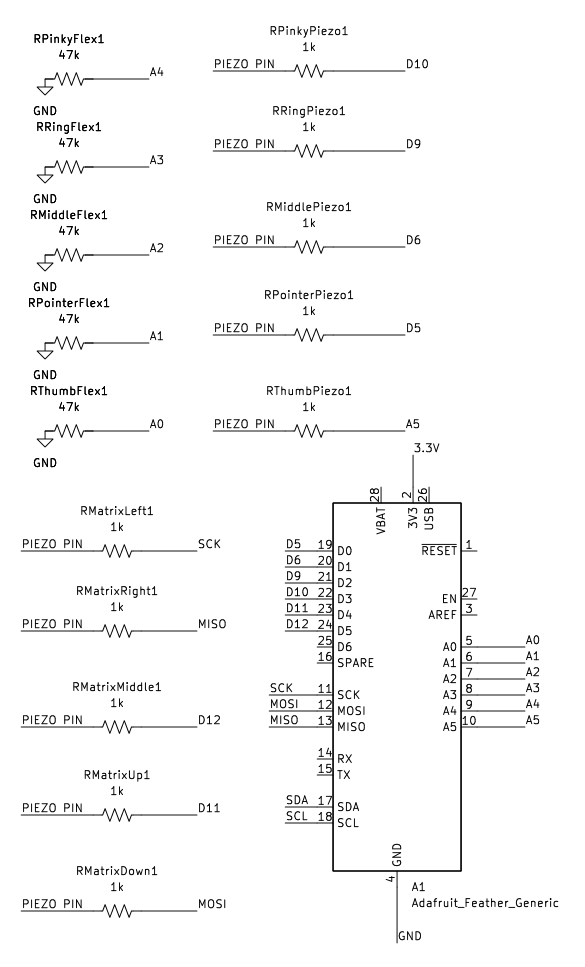
\includegraphics[height=6.9in]{../pcb/exports/pcb-schematic-preview.png}
\caption{October 22 KiCad connection draft, exported from the team's saved
schematic~\cite{repo}. It shows flex-resistor branches and tentative ten-piezo
connections, not the complete as-built circuit. The generic Feather symbol,
board-specific pins, repeated piezo net labels and missing sensor/driver circuits
require review before layout.}
\label{fig:schematic}
\end{figure}

\par\Needspace{3.5in}
\begin{center}
\small
\begin{tabularx}{\linewidth}{@{}P{3.1cm}P{2.4cm}Y@{}}
\toprule
\textbf{Date/window} & \textbf{State} & \textbf{Milestone / dependency}\\
\midrule
September 10--17 & Recorded & Alpha builds/tests; real static recording/export pilot.\\
October 2--6 & Demonstrated & Account/practice implementation, recorded model training and phone integration; sign completion and database progress observed. Controlled live validation incomplete.\\
October 22--28 & In progress & KiCad schematic/layout planning and TCN review; glove remains on perfboard. Piezo elements and ICM-20948 received; flex repair awaited.\\
Next two weeks & Planned & Replace/calibrate flex sensors; integrate ICM-20948; complete circuit/driver design and initial haptic cues. Sequence depends on delivery and bench checks.\\
Before November 19 & Proposed target & Collect fresh trials, evaluate revised features/model, verify live practice and progress, and test cue perception.\\
November 19 & Scheduled & Post-mortem presentation.\\
December 3 & Tentative & Evening CpE Showcase, approximately 6 p.m., WERT Lobby.\\
\bottomrule
\end{tabularx}
\captionsetup{hypcap=false}
\captionof{table}{Completed work and team-reported roadmap as of October 28.
Future engineering dates are targets.}
\label{tab:timeline}
\end{center}

Repair will establish per-finger ranges before new data collection. IMU work
will verify all nine channels and compare calibrated fusion against a baseline,
preserving meaningful palm orientation. New input features require matching
training and phone preprocessing. Haptic work must connect a defined correction
signal to bounded actuator commands and validate perception with sensors
monitored both during and after activation. Final checks should include wrong
signs, idle motion, disconnects, restart, account isolation and repeated latency
measurements. Independent trials and held-out users are needed before broader
recognition claims. Piezo drive specifications, mounting and tactile suitability
still need verification.

\par\Needspace{10\baselineskip}
\section{Conclusion}
Helping Hand integrates wearable sensing, saved practice, recording tools and
a compact three-word TCN. Software checks, offline experiments and team-reported
demonstrations support the prototype; live reliability, generalization and
learning benefits require further evaluation. Despite sensor damage, circuit
planning and model review have continued. The next phase will calibrate the
repaired glove, integrate the received ICM-20948, evaluate recognition changes
and prototype directional piezo cues. Reproducible system/user tests and ASL
community expertise should guide future vocabulary and feedback development.
% BODY END

\clearpage
\begin{thebibliography}{99}
\small
\raggedright
\setlength{\itemsep}{3pt}
\bibitem{nidcd} NIDCD, ``American Sign Language.'' \url{https://www.nidcd.nih.gov/health/american-sign-language}. Accessed Oct. 27, 2026.
\bibitem{design} Helping Hand team, \emph{Helping Hand Design Draft}, first-semester design report. \href{https://github.com/GG1627/helping-hand/blob/a35d0f5/design_draft/Helping_Hand_Design_Draft.pdf}{Project design archive}, 2026.
\bibitem{educators} S. Hassan et al., ``ASL Educators' Perspectives on AI for Enhancing Student Learning in American Sign Language Education,'' \emph{CHI}, 2026, 20 pp. \href{https://doi.org/10.1145/3772318.3791928}{doi:10.1145/3772318.3791928}.
\bibitem{lee} B. G. Lee, T.-W. Chong and W.-Y. Chung, ``Sensor Fusion of Motion-Based Sign Language Interpretation with Deep Learning,'' \emph{Sensors}, 20(21), 6256, 2020. \href{https://doi.org/10.3390/s20216256}{doi:10.3390/s20216256}.
\bibitem{tcn} S. Bai, J. Z. Kolter and V. Koltun, ``An Empirical Evaluation of Generic Convolutional and Recurrent Networks for Sequence Modeling,'' author preprint, 2018. \url{https://arxiv.org/abs/1803.01271}.
\bibitem{quaternion} A. Yurtman, B. Barshan and B. Fidan, ``Activity Recognition Invariant to Wearable Sensor Unit Orientation Using Differential Rotational Transformations Represented by Quaternions,'' \emph{Sensors}, 18(8), 2725, 2018. \href{https://doi.org/10.3390/s18082725}{doi:10.3390/s18082725}.
\bibitem{magnetic} M. Kok and T. B. Sch\"on, ``Magnetometer Calibration Using Inertial Sensors,'' \emph{IEEE Sensors Journal}, 16(14), pp. 5679--5689, 2016. \href{https://doi.org/10.1109/JSEN.2016.2569160}{doi:10.1109/JSEN.2016.2569160}.
\bibitem{hapticstudy} M. Tajdari, J. Forsyth and S. Lim, ``Sensitivity to Vibrotactile Stimulation in the Hand and Wrist: Effects of Motion, Temporal Patterns, and Biological Sex,'' \emph{Human Factors}, 67(4), pp. 331--346, 2025; first online Aug. 23, 2024. \href{https://doi.org/10.1177/00187208241275734}{doi:10.1177/00187208241275734}.
\bibitem{ble} Bluetooth SIG, ``The Bluetooth Low Energy Primer,'' ATT/GATT and notification sections. \url{https://www.bluetooth.com/bluetooth-le-primer/}.
\bibitem{nus} Nordic Semiconductor, ``Nordic UART Service (NUS).'' \url{https://nrfconnectdocs.nordicsemi.com/ncs/latest/nrf/libraries/bluetooth/services/nus.html}.
\bibitem{staticrecord} Helping Hand team, \emph{Recorded Static MLP for the October 6 Demo}, Oct. 6, 2026. \href{https://github.com/GG1627/helping-hand/blob/a35d0f5/docs/STATIC_MLP_DEMO_MODEL.md}{Versioned training, calibration and verification record}.
\bibitem{wordrecord} Helping Hand team, \emph{Recorded Word Demo Model}, Oct. 5, 2026. \href{https://github.com/GG1627/helping-hand/blob/a35d0f5/docs/WORD_MODEL_DEMO_TRAINING.md}{Versioned dataset, split, training and evaluation record}.
\bibitem{integration} Helping Hand team, \emph{TCN Word Practice Integration}, Oct. 5, 2026. \href{https://github.com/GG1627/helping-hand/blob/a35d0f5/docs/WORD_DEMO_INTEGRATION.md}{Versioned integration and software-verification record}.
\bibitem{auth} Firebase, ``Authenticate with Firebase using password-based accounts on Flutter.'' \url{https://firebase.google.com/docs/auth/flutter/password-auth}.
\bibitem{firestore} Firebase, ``Writing conditions for Cloud Firestore Security Rules.'' \url{https://firebase.google.com/docs/firestore/security/rules-conditions}.
\bibitem{cloudsecurity} Firebase, ``Privacy and Security in Firebase,'' data protection in transit. \url{https://firebase.google.com/support/privacy/}. Accessed Oct. 28, 2026.
\bibitem{piezo} TIMESETL, piezo pickup-disc seller listing, Amazon ASIN B077YJ3H6R, \url{https://www.amazon.com/dp/B077YJ3H6R}, accessed Oct. 28, 2026; purchased-product match confirmed by the team. Drive ratings unverified. Murata, \href{https://www.murata.com/en-global/support/faqs/sound/diaphragm/char/sch0001}{External-drive piezoelectric diaphragm circuit guidance}, general background, not this part's datasheet.
\bibitem{flex} Adafruit Industries, ``Short Flex Sensor,'' product 1070, \url{https://www.adafruit.com/product/1070}; Spectra Symbol, \emph{Flex Sensor Datasheet}, Rev. A2, \url{https://cdn-shop.adafruit.com/datasheets/SpectraFlex2inch.pdf}. Accessed Oct. 27, 2026.
\bibitem{repo} Helping Hand team, \emph{Helping Hand Repository}: source, README, firmware configuration, recorded exports and KiCad files; snapshot \texttt{a35d0f5}, Oct. 27, 2026. \url{https://github.com/GG1627/helping-hand/tree/a35d0f5}.
\bibitem{platformio} PlatformIO, ``What is PlatformIO?'' \url{https://docs.platformio.org/en/latest/what-is-platformio.html}.
\bibitem{flutter} Flutter, ``Flutter documentation.'' \url{https://docs.flutter.dev/}.
\bibitem{keras} TensorFlow, ``Keras: The high-level API for TensorFlow.'' \url{https://www.tensorflow.org/guide/keras}.
\bibitem{litert} Google AI Edge, ``LiteRT for Microcontrollers.'' \url{https://developers.google.com/edge/litert/microcontrollers/overview}.
\bibitem{scaler} scikit-learn, ``StandardScaler.'' \url{https://scikit-learn.org/stable/modules/generated/sklearn.preprocessing.StandardScaler.html}.
\bibitem{pytest} pytest, ``pytest documentation.'' \url{https://docs.pytest.org/en/stable/}.
\bibitem{fluttertests} Flutter, ``Testing Flutter apps.'' \url{https://docs.flutter.dev/testing/overview}.
\bibitem{kicad} KiCad, \emph{Getting Started in KiCad}, reference documentation. \url{https://docs.kicad.org/9.0/en/getting_started_in_kicad/getting_started_in_kicad.html}. Reference version does not identify the team's installed release.
\bibitem{git} Git, ``git documentation.'' \url{https://git-scm.com/docs/git}.
\bibitem{i2c} NXP, \emph{I2C-bus Specification and User Manual}, UM10204, Rev. 7.0, Oct. 1, 2021. \url{https://www.nxp.com/docs/en/user-guide/UM10204.pdf}.
\bibitem{imu} Adafruit Industries, ``TDK InvenSense ICM-20948 9-DoF IMU,'' product 4554, \url{https://www.adafruit.com/product/4554}; \emph{ICM-20948 Arduino Guide}, \url{https://learn.adafruit.com/adafruit-tdk-invensense-icm-20948-9-dof-imu/arduino}. Accessed Oct. 27, 2026.
\bibitem{sme} Helping Hand team, \emph{Our Findings from the ASL Glove Demos}, remote Notre Dame ASL-club discussion notes, recorded date Sept. 18, 2026 with incomplete fields. \href{https://github.com/GG1627/helping-hand/blob/a35d0f5/SME.md}{Versioned formative-feedback notes}.
\bibitem{deafled} A. Desai et al., ``Systemic Biases in Sign Language AI Research: A Deaf-Led Call to Reevaluate Research Agendas,'' \emph{LREC-COLING SignLang Workshop}, pp. 54--65, 2024. \url{https://aclanthology.org/2024.signlang-1.6/}.
\bibitem{ewaste} ITU/UNITAR, \emph{Global E-waste Monitor 2024}, 2024. \href{https://www.itu.int/en/publications/ITU-D/pages/publications.aspx?media=electronic&parent=D-GEN-E_WASTE.01-2024}{Official publication record}.
\bibitem{ethics} IEEE, ``IEEE Code of Ethics.'' \url{https://ieee-cas.org/about/ieee-code-ethics}.
\bibitem{pilot} Helping Hand team, \emph{Static ASL Pilot Recording}, Sept. 17, 2026. \href{https://github.com/GG1627/helping-hand/tree/a35d0f5/backend/recorded_data}{Raw exports and dataset description}.
\bibitem{demoobservations} Helping Hand team, \emph{October 5--6 Demonstration Observations}, reported Oct. 28, 2026: NSC senior design lab, Fairphone Gen 6/Android 15 reference configuration. Retrospective account in the repository's R3 demonstration notes; controlled trial logs and detailed software revisions unavailable.
\bibitem{testplans} Helping Hand team, \emph{T1 Alpha Test Plan} and \emph{T2 Beta Test Plan}, Sept.--Oct. 2026. \href{https://github.com/GG1627/helping-hand/blob/a35d0f5/docs/T1_ALPHA_TEST_PLAN.md}{T1 procedures}; \href{https://github.com/GG1627/helping-hand/blob/a35d0f5/docs/T2_Beta_Test_Plan.tex}{T2 procedures and run-record requirements}.
\bibitem{review} Helping Hand team with Codex assistance, \emph{R3 TCN Improvement Review}, Oct. 27, 2026. \href{https://github.com/GG1627/helping-hand/blob/a35d0f5/docs/R3_TCN_IMPROVEMENT_REVIEW.md}{Current code-review findings; no new experimental result}.
\end{thebibliography}
\end{document}
